\documentclass [memoire, letterpaper, oneside, 12pt]{thETS-utf8}

\listfiles

\usepackage{palatino}
\usepackage[round]{natbibETS} %Pour faire les citations du genre Autheur (Année)
% Pour faire une citation du genre Auteur (Année), utilisez la commande \citet

%%%%%%%%%%%%%%%%%%%%%%%%%%%%%%%%%%%%%%%%%%%%%%%%%%%%%%%%%%%%%%%%
\usepackage{multibib} %Pour faire la liste des références
\newcites{refs}{LISTE DE RÉFÉRENCES}
%%%%%%%%%%%%%%%%%%%%%%%%%%%%%%%%%%%%%%%%%%%%%%%%%%%%%%%%%%%%%%%%

\usepackage{mathptmx}
\usepackage{times}
\usepackage{amsmath}  % Symboles et fonctions math\'eatiques suppl\'eentaires
\usepackage{amssymb}  % Symboles math\'eatiques
\usepackage{amsfonts}
\usepackage[utf8]{inputenc}
\usepackage{graphicx}
\usepackage{color}
\usepackage[T1]{fontenc}
\usepackage{subfig}
\usepackage{setspace}
\usepackage{float}
\usepackage[round]{natbibETS}
\usepackage{varwidth}
\usepackage[section]{placeins}
\usepackage[mathcal]{euscript}
\usepackage{enumerate}
\usepackage{tikz}
\usepackage{import}
\usepackage{todonotes}
\usepackage{MyAlgorithmic}
\usepackage[boxed,chapter]{MyAlgorithm}
\usepackage{nameref}
\usepackage{multirow}
\usepackage{caption}
\usepackage{listings}
\usepackage{textcomp}
\usepackage{hyperref}
\usepackage{minibox}

\hypersetup{
    colorlinks=true,    % false: boxed links; true: colored links
    linkcolor=black,    % color of internal links
    citecolor=black,    % color of links to bibliography
    filecolor=black,    % color of file links
    urlcolor=blue      % color of external links
}

\newcommand{\LT}[1]{%
	{
	\todo[inline,color={red!33!green!33!blue!33}]{%
	\textbf{[LT]:}~#1}
	}}
	
\newcommand{\SC}[1]{%
	{
	\todo[inline,color={red!100!green!33!}]{%
	\textbf{[SC]:}~#1}
	}}

\newcommand{\fig}[1]{figure~\ref{#1}}
\newcommand{\ang}[1]{(\textit{#1})}
\newcommand{\bul}{$\quad\bullet$~~}
\newcommand{\ltCodec}{logiciel de référence H.264/AVC JM}
\newcommand{\sect}[1]{section~\ref{#1}}
\newcommand{\page}[1]{(p.~\pageref{#1})}

\newcommand{\ltSAD}[1]{\textrm{SAD}(#1)}
\newcommand{\ltMIN}[1]{\arg \min_{#1}}
\newcommand{\lttBLK}[2]{\textrm{MCB}_{#1}(#2)}
\newcommand{\ltCB}[2]{\mathbf{b}_{#1}(#2)}
\newcommand{\ltSTBLK}[1]{\textrm{SMCB}(#1)}
\newcommand{\ltBor}[1]{\mathcal{#1}}

\newcommand{\ltSDMCB}[1]{\textrm{SDMCB}(#1,\ltP{},m,n)}
\newcommand{\ltErr}[1]{\mathbf{\hat{F}}_{#1}}
\newcommand{\ltConc}[1]{\mathbf{F^{\prime}}_{#1}}
\newcommand{\ltOpt}[1]{\mathbf{F^{*}}_{#1}}

\newcommand{\ltF}[1]{\mathbf{F}_{#1}}
\newcommand{\ltE}[1]{\mathbf{E}_{#1}}
\newcommand{\ltP}[1]{\mathbf{P}_{#1}}
\newcommand{\ltD}[1]{\mathbf{D}_{#1}}
\newcommand{\ltS}[1]{I_{#1}}

\newcommand{\ltDiffGood}{\left| \ltF{x,y} - \ltP{x,y} \right|}

\hyphenpenalty=5000
\tolerance=1000

\definecolor{listinggray}{gray}{0.9}
\definecolor{lbcolor}{rgb}{0.9,0.9,0.9}
\lstset{
	backgroundcolor=\color{white},
	tabsize=4,
	rulecolor=,
	language=matlab,
    basicstyle=\tiny,
    upquote=true,
    columns=fixed,
    showstringspaces=false,
    extendedchars=true,
    breaklines=true,
    prebreak = \raisebox{0ex}[0ex][0ex]{\ensuremath{\hookleftarrow}},
    frame=single,
    showtabs=false,
    showspaces=false,
    showstringspaces=false,
    identifierstyle=\ttfamily,
    keywordstyle=\color[rgb]{0,0,1},
    commentstyle=\color[rgb]{0.133,0.545,0.133},
    stringstyle=\color[rgb]{0.627,0.126,0.941},
}

\captionsetup[algorithm]{labelfont=normalfont,labelsep=quad,justification=centering,skip=1cm}
%\usepackage[pdftex]{hyperref}


%%%%%%%%%%%%%%%%%%%%%%%%%%%%%%%%%%%%%%%%%%%%%%%%%%%%%%%%%%%%%%%%%%%%%%%%%%%%%%%%%%%%%%%%%%%%%%%
%%
%%   IMPORTANT
%%
%%  Si vous créez un fichier PDF directement avec PDFLatex, et vous utilisez Acrobat Reader
%% pour faire l'impression, n'oubliez-pas de changer l'option <<Mise à l'échelle>> pour la valeur
%% <<Aucune>> pour que les marges soient imprimés correctement.
%%
%%%%%%%%%%%%%%%%%%%%%%%%%%%%%%%%%%%%%%%%%%%%%%%%%%%%%%%%%%%%%%%%%%%%%%%%%%%%%%%%%%%%%%%%%%%%%%%%%%%%

\listfiles

%------------------------------------------------------------------------------------------------------------------------------------------

% à décommanter et modifier si nécessaire dans le cas d'une maitrise
\genie{Des technologies de l'information}
%\diplome{
%  DE LA\\
%  MAÎTRISE EN GÉNIE DES TECHNOLOGIES DE L'INFORMATION\\
%  M.Ing.
%}

\title{Détection et dissimulation de la détérioration visuelle issue du décodage
de séquences H.264 corrompues}

\author{Luc TRUDEAU}
\authorcopyright{Luc Trudeau}

\datesoutenance{16 Mai 2011}

\datedepot{\today}

\directeur{M.}{Stéphane Coulombe}{Département de génie logiciel et des TI à
l'École de technologie supérieure}

\president{M.}{Mohamed Cheriet}{Département de génie de la production automatisée à l’École de technologie supérieure}

\jury{M.}{Luc Duong}{Département de génie logiciel et des TI à l'École de
technologie supérieure}{}

%\examinexterne{M.}{Prénom Nom}{département et institution}{}

%---------------------------------------------------------------------------------
%---------------------------------------------------------

\begin{document}

\pagenumbering{Roman}

%%%%%%%%%%%%%%%%%%%%%%%%%%%%%%%%%%%%%%%%%%%%%%%%%%%
% PAGE TITRE
%%%%%%%%%%%%%%%%%%%%%%%%%%%%%%%%%%%%%%%%%%%%%%%%%%%
\maketitle
%%%%%%%%%%%%%%%%%%%%%%%%%%%%%%%%%%%%%%%%%%%%%%%%%%%
% PRÉSENTATION JURY
%%%%%%%%%%%%%%%%%%%%%%%%%%%%%%%%%%%%%%%%%%%%%%%%%%%
\presentjury

%%%%%%%%%%%%%%%%%%%%%%%%%%%%%%%%%%%%%%%%%%%%%%%%%%%
% AVANT PROPOS
%%%%%%%%%%%%%%%%%%%%%%%%%%%%%%%%%%%%%%%%%%%%%%%%%%%
%\begin{avantpropos}
%Facultatif
%\end{avantpropos}

% %%%%%%%%%%%%%%%%%%%%%%%%%%%%%%%%%%%%%%%%%%%%%%%%%% REMERCIEMENTS
% %%%%%%%%%%%%%%%%%%%%%%%%%%%%%%%%%%%%%%%%%%%%%%%%%%
\begin{remerciements}
Ce mémoire de maîtrise fait le point sur certains concepts proéminents issus de
plus de 2 ans de recherche sur la détection et la dissimulation
d’erreurs. Vous conviendrez avec moi qu’un tel effort de recherche requiert des
ressources financières et matérielles considérables. C’est pourquoi j’exprime ma
reconnaissance et mes remerciements à Stéphane Coulombe, professeur à l’École de
technologie supérieure, qui a accepté de me faire confiance dans ce projet et
d’avoir consacré les ressources nécessaires à sa réalisation. J’en profite
également pour souligner son engagement hors du commun en ce qui a trait à ma
formation et à la qualité de ce mémoire.

Je tiens à remercier Evelyne, ma conjointe, qui m’a toujours soutenu dans cette
aventure, à tous les niveaux. À nos deux filles, Joannie et Alexane, qui tout
comme Evelyne, sont pour moi une source de motivation inépuisable.

Je tiens à souligner les efforts de Chantal Gamache, conseillère au Service
d'appui en communication (SAC) à l’École de technologie supérieure, et Steven
Pigeon, professionnel de recherche à la chaire de recherche industrielle Vantrix
en optimisation vidéo. Chantal a consacré son temps, sa patience et son talent à
l’amélioration de la qualité de la rédaction de cet ouvrage. Steven, de par son
savoir-faire et ses connaissances, a enrichi, lors de nos nombreux échanges, mon
approche et mes méthodes de recherches.

Finalement, cet ouvrage fut rendu possible, en partie, par le Conseil de
recherches en sciences naturelles et en génie du Canada (CRSNG), bourse
\#356807-07 et, en partie, par Le Fonds québécois de la recherche sur la nature
et les technologies (FQRNT), bourse \#141698.
\end{remerciements}

% %%%%%%%%%%%%%%%%%%%%%%%%%%%%%%%%%%%%%%%%%%%%%%%%%% SOMMAIRE
% %%%%%%%%%%%%%%%%%%%%%%%%%%%%%%%%%%%%%%%%%%%%%%%%%%
\motscles{Détection d'erreurs, dissimulation d'erreurs, H.264, vidéo mobile.}
\begin{sommaire}
Compte tenu de leur nature, les réseaux mobiles sont plus fortement enclins à la
corruption de données que leurs contreparties filaires. Même si les données se
rendent à destination, les bits endommagés entrainent le rejet des paquets qui
les encapsulent. Ces pertes ont un impact important sur la qualité de
l'expérience de l'utilisateur lors de la consultation de flux vidéos ou de la
vidéophonie, et ce, surtout lorsque la retransmission n'est pas envisageable. On
restreint l'usage des approches conventionnelles de résilience aux erreurs, tels
la retransmission de trames ou l'ajout de trames redondantes, car elles imposent
un fardeau considérable aux réseaux mobiles, ceux-ci étant déjà fortement
achalandés.

Dans cet ouvrage, nous proposons la réutilisation sélective des données
corrompues afin d'augmenter la qualité visuelle de séquences endommagées. Cette
sélection est guidée par une nouvelle approche de détection de la détérioration
visuelle dans le domaine des pixels. Elle combine la mesure des effets de bloc
(discontinuités spatiales en bordure de blocs) à l'estimation du mouvement.

Notre méthode a été testée sur un ensemble de 17 séquences QCIF codées en H.264
avec des QP de 16 à 28 et soumis à des taux d'erreurs de 0.0004 à 0.0032. Nos
résultats de simulation démontrent qu'il est possible de décoder des trames
corrompues. La probabilité d’un décodage réussi varie de 20~\% à 70~\% selon les
paramètres d’encodage et le taux d’erreurs subies lors du transport. De plus,
notre algorithme, développé en fonction de la norme H.264, réussit à effectuer
le bon choix de 81~\% à 86~\% et 88~\% à 91~\% des cas (selon les conditions).
Lorsque que notre algorithme est combiné au décodeur de référence H.264, nous
observons un gain moyen 0.65 dB à 0.86 dB de PSNR (selon les conditions).
\end{sommaire} 

% %%%%%%%%%%%%%%%%%%%%%%%%%%%%%%%%%%%%%%%%%%%%%%%%%% ABSTRACT
% %%%%%%%%%%%%%%%%%%%%%%%%%%%%%%%%%%%%%%%%%%%%%%%%%%
\keywords{Error concealment, error detection, H.264, mobile video, pixel domain}
\begin{abstract}{Detection and concealment of visual degradation resulting from
erroneous H.264 sequences} In mobile video applications, where unreliable
networks are commonplace, corrupted video packets can have a profound impact on
the quality of the user experience. Error resilient mechanisms like
retransmission and redundant frames may impose an unacceptable burden on mobile
networks. In these cases a decoder-based error resilience approach, like the one
described in this work, can help improve the end-user experience without adding
load to the network.

In this master's thesis, we show that, in a wide range of operating conditions,
selectively reusing data resulting from decodable broken packets leads to better
results than frame copy. This selection is guided by a novel concept that
combines motion estimation and a measure of blocking artefacts at block edges to
predict visual degradation caused by the decoding of erroneous packets.

The proposed solution was tested against 17, H.264 coded, QCIF sequence with
quantization parameters from 16 to 28 and exposed to bit error rates of 0.0004
to 0.0032. Simulation results show that the probability of successfully decoding
a broken sequence varies from 20~\% to 70~\% (depending on operating
conditions). Combined with the proposed solution, the H.264/AVC JM reference
software decoder can select the best option between frame copy and the erroneous
frame decoding in 81~\% to 86~\% and 88~\% to 91~\% of the test cases (depending
on operating conditions). We also obtain an average gain of 0.65~dB to 0.86~dB
(depending on operating conditions).
\end{abstract}

%%%%%%%%%%%%%%%%%%%%%%%%%%%%%%%%%%%%%%%%%%%%%%%%%%%
% TABLE DES MATIÈRES
%%%%%%%%%%%%%%%%%%%%%%%%%%%%%%%%%%%%%%%%%%%%%%%%%%%
\tableofcontents

%%%%%%%%%%%%%%%%%%%%%%%%%%%%%%%%%%%%%%%%%%%%%%%%%%%
% LISTE DES TABLEAUX
%%%%%%%%%%%%%%%%%%%%%%%%%%%%%%%%%%%%%%%%%%%%%%%%%%%
\listoftables

%%%%%%%%%%%%%%%%%%%%%%%%%%%%%%%%%%%%%%%%%%%%%%%%%%%
% LISTE DES FIGURES
%%%%%%%%%%%%%%%%%%%%%%%%%%%%%%%%%%%%%%%%%%%%%%%%%%%
\listoffigures

%%%%%%%%%%%%%%%%%%%%%%%%%%%%%%%%%%%%%%%%%%%%%%%%%%%
% LISTE DES EXTRAITS DE CODE
%%%%%%%%%%%%%%%%%%%%%%%%%%%%%%%%%%%%%%%%%%%%%%%%%%%
%\lstlistoflistings

%%%%%%%%%%%%%%%%%%%%%%%%%%%%%%%%%%%%%%%%%%%%%%%%%%%
% LISTE DES ABBREVIATIONS
%%%%%%%%%%%%%%%%%%%%%%%%%%%%%%%%%%%%%%%%%%%%%%%%%%%
\begin{listofabbr}[3cm] 
\item [AIDB] \textit{Average Inter-sample Difference across Boundaries}
\item [AIDSB] \textit{Average Internal Difference between Subsequent Blocks}
\item [ASO] \textit{Arbitrary Slice Order}
\item [AVC] \textit{Advanced video coding}
\item [BER] \textit{Bit error rate}\\ Taux d'erreurs binaire
\item [CABAC] \textit{Context-adaptive binary arithmetic coding}\\ Codage
arithmétique binaire à contexte adaptatif
\item [CAVLC] \textit{Context-adaptive variable-length coding}\\ Codage
entropique à longueur variable
\item [COD] Bit positionné en début de macrobloc identifiant s'il est encodé ou
pas.
\item [dB] décibel
\item [DCT] \textit{Discrete cosine transform}\\ Transformée en cosinus discrète
\item [FMO] \textit{Flexible macroblock ordering}\\ Ordonnancement flexible de
macroblocs.
\item [IAIDB] \textit{Internal AIDB}
\item [${IAIDB}_{block}$] \textit{Internal AIDB per block}
\item [IP] \textit{Internet protocol}\\ Protocole Internet
\item [JM] \textit{Joint Model}
\item [JPEG] \textit{Joint photographic experts group}
\item [ko/s] Kilooctet par seconde
\item [LBP] \textit{Local binary pattern}\\ Patron binaire local
\item [MCB] \textit{Motion compensated blockiness}\\ Effets de bloc compensés
par le mouvement
\item [MPEG] \textit{Moving picture experts group}
\item [NAL] \textit{Network abstraction layer}\\ Couche d'abstraction réseau
\item [OSI] \textit{Open Systems Interconnection}
\item [PMVFAST] \textit{Predictive Motion Vector Field Adaptive Search
Technique}
\item [PSNR] \textit{Peak signal-to-noise ratio}
\item [QCIF] \textit{Quarter common international format} ($176 \times 144$)
\item [QP] \textit{Quantization parameter}\\ Paramètre de quantification
\item [RBSP] \textit{Raw Byte Sequence Payload}
\item [RTP] \textit{Real-time transport protocol}\\ Protocole de streaming
temps-réel
\item [SAD] \textit{Sum of absolute differences}\\ Somme des différences
absolues
\item [SAE] \textit{Sum of absolute error}\\ Somme de l'erreur absolue
\item [SDMCB] \textit{Sum of the distributed motion compensated blockiness}
\\ Somme des effets de bloc compensés par le mouvement distribuée
\item [SMCB] \textit{Sum of motion compensated blockiness}\\ Somme des effets de
bloc compensés par le mouvement
\item [SVM] \textit{Support vector machine}\\ Machine à vecteurs de support.
\item [TC] \textit{Texture consistancy}\\ Consistance de la texture
\item [UMHexagonS] \textit{Unsymmetrical cross Multi-Hexagon-Grid-Search}
\item [UDP] \textit{User datagram protocol}\\ Protocole de datagramme
utilisateur
\item [VCL] \textit{Video coding layer}\\ Couche de codage vidéo
\item [$YC_BC_R$] Luminance, chrominance bleu, chrominance rouge
\end{listofabbr}


%%%%%%%%%%%%%%%%%%%%%%%%%%%%%%%%%%%%%%%%%%%%%%%%%%%
% LISTE DES SYMBOLES
%%%%%%%%%%%%%%%%%%%%%%%%%%%%%%%%%%%%%%%%%%%%%%%%%%%
%\begin{listofsymbols}[3cm]
%\item [$\beta$] Paramètre de l'algorithm
%\item [$A$] Ça n'importe pas
%\item [$\xi$] Ça n'importe pas

%\end{listofsymbols}

%%%%%%%%%%%%%%%%%%%%%%%%%%%%%%%%%%%%%%%%%%%%%%%%%%%
% CORPS DE LA THÈSE
%%%%%%%%%%%%%%%%%%%%%%%%%%%%%%%%%%%%%%%%%%%%%%%%%%%


\reversemarginpar % pour que les marginpar s'amenent a GAUCHE du doc.

\begin{introduction}
\pagenumbering{arabic}
\import{Intro/}{intro.tex}
\end{introduction}

\import{H264/}{h264.tex}
\import{H264Transport/}{H264Transport.tex}
\import{Erreurs/}{erreurs.tex}
\import{RevueLit/}{revueLit.tex}
\import{MCB/}{mcb.tex}
\import{Resultats/}{resultats.tex}

\begin{conclusion}
\import{Conclusion/}{conclusion.tex}
\end{conclusion}


%%%%%%%%%%%%%%%%%%%%%%%%%%%%%%%%%%%%%%%%%%%%%%%%%%%
%  ANNEXE:
%%%%%%%%%%%%%%%%%%%%%%%%%%%%%%%%%%%%%%%%%%%%%%%%%%%
\appendix
\multiannexe % si on a plus d'une annexe
%\include{annexe1}
\captionsetup{list=no}
\begin{chapter}{Configuration du banc d'essai}
\label{Ann-Setup}

La \fig{fig-Setup} décrit les différentes étapes de traitement de notre banc
d'essai. Ce diagramme permet d'établir le lien entre les
figures~\ref{fig-EncoderDecoder} et \ref{fig-SelectiveSetup} de la section
<<~\nameref{chap-resultats}~>>.
\begin{figure}[h]
	\fbox{ % cette commande est nécéssaire pour encadrer les figures
	\centering
		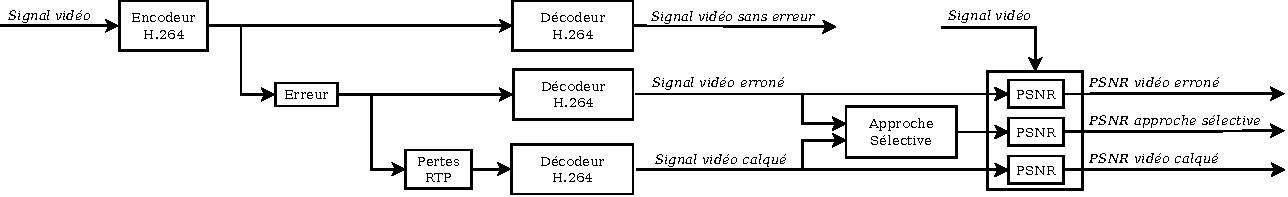
\includegraphics[angle=90, height=0.54\paperheight]{Annexe/Setup.pdf}
	}
	\caption{Configuration du banc d'essai utilisé pour réaliser
	l'expérimentation.}
	\label{fig-Setup}
\end{figure}
\end{chapter}


\begin{chapter}{Résultats détaillés de simulations}
\label{Ann-Simulation}


\import{Annexe/}{parSequence.tex}
\import{Annexe/}{toutesSequences.tex}

\end{chapter}

\begin{chapter}{Code source}
\import{Annexe/}{codeSource.tex}
\end{chapter}

%%%%%%%%%%%%%%%%%%%%%%%%%%%%%%%%%%%%%%%%%%%%%%%%%%%
% LISTE DE RÉFERENCES
%
% IMPORTATANT:
% Pour que ça marche:
%   1. Compiler le document une fois
%   2. Rouler la commande: << bibtex refs >>...cliquer sur le fichier update_refs.bat sur Windows
%   3. Recompiler le document
%%%%%%%%%%%%%%%%%%%%%%%%%%%%%%%%%%%%%%%%%%%%%%%%%%%

%Changement d'interligne pour passer en simple pour les références et la bibliographie.

%\newpage
\singlespacing
\nociterefs{*} %Ici vous devez inclure les références qui ne sont pas cités, ou étoiles pour toutes les réfs
\bibliographystylerefs{bibETS}
\addcontentsline{toc}{chapter}{LISTE DE RÉFÉRENCES}
\bibliographyrefs{biblio} % à décommander et indiquer la liste des fichiers bib
\doublespacing

%------------------------------------------------------------------------------------------------------------------------------------------


%%%%%%%%%%%%%%%%%%%%%%%%%%%%%%%%%%%%%%%%%%%%%%%%%%%
% BIBLIOGRAPHIE
%%%%%%%%%%%%%%%%%%%%%%%%%%%%%%%%%%%%%%%%%%%%%%%%%%%
\newpage
\singlespacing
\bibliographystyle{bibETS}
\addcontentsline{toc}{chapter}{BIBLIOGRAPHIE}
\bibliography{memoire} % à décommander et indiquer la liste des fichiers bib
\doublespacing

\end{document}
